%\let\textcircled=\pgftextcircled
\chapter{Trajectory integration}
\label{chap:trajectory_integration}

Initially I coded both square, trapezoid and the parabola method, that from now one will be called PaIS, for analyzing what better suited my necessities. \cite{casciola} \\
A quadrature formula of grade $n$ provides the exact integral value of a polynomial of grade $\leq n$, which means that it isn't always the best choice to use a formula with a high grade. \\
\\
\justify
I verified experimentally the difference in error between integration methods by creating a synthetic trajectory.
\begin{figure}[H]
\centering
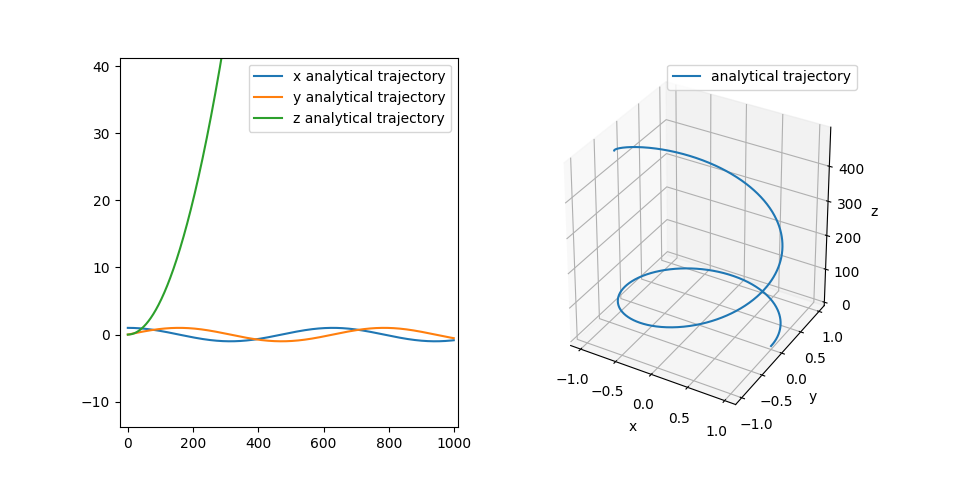
\includegraphics[scale=0.6]{spring.png}
\caption{Trajectory created to evaluate integration error}
\end{figure}
\justify
then i compared the integrated one with the analytical.
\begin{figure}[H]
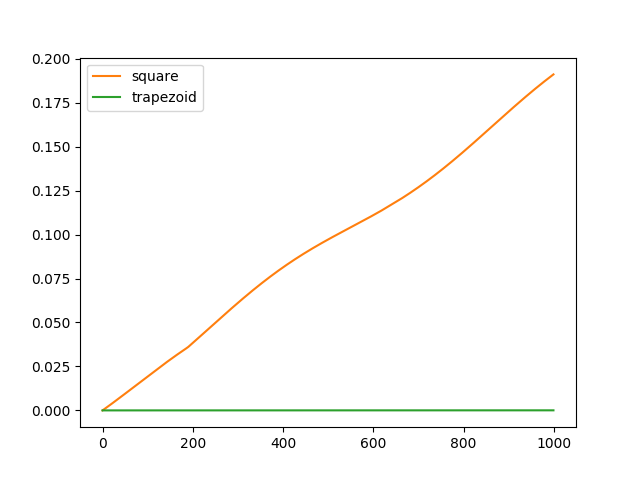
\includegraphics[width=\textwidth/2]{square_vs_trapezoid.png}
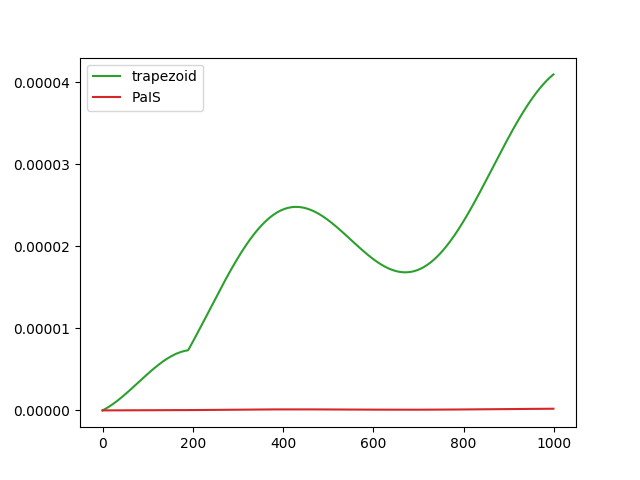
\includegraphics[width=\textwidth/2]{trapezoid_vs_PaIS.png}
\caption{Absolute error from analytical trajectory}
\end{figure}

\justify
Numpy offers a compact way to write operation even in large arrays. This is for example trapezoid method in one line.

\begin{lstlisting}[language=Python,frame=single,basicstyle=\footnotesize]
def trapz_integrate_delta(times, vector):
    return (((vector[:,:-1] + vector[:,1:]) * (times[1:]-times[:-1])) * 0.5).cumsum()
\end{lstlisting}

Difference between PaIS and trapezoid can be seen after integrating for about 11 minutes.
\begin{figure}[H]
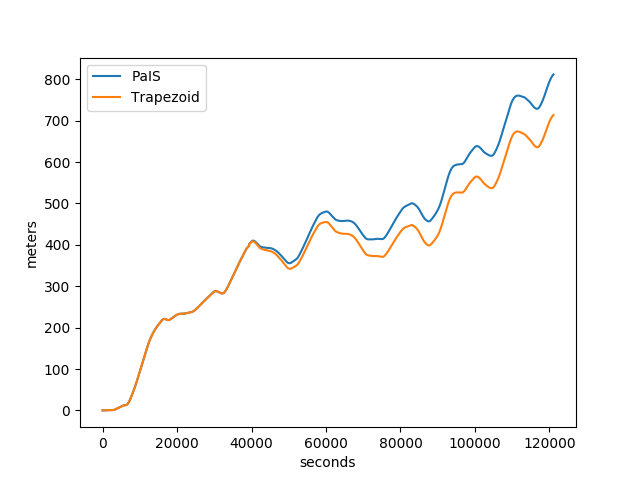
\includegraphics[scale=0.6]{trapezoid_vs_Pais_real_world.png}
\caption{Difference between trapezoid and PaIS method on real world data}
\end{figure}

\justify
I decided to use PaIS because measures in discrete time produce a function $C^0$ while physics quantities of a vehicle in continuous time are at least $C^1$, 
\justify
But still the error was too large, the integrated trajectory diverge after some time by moving away too much from the ideal real trajectory.
So i improved integrated trajectory with GNSS data that is more precise but has a lower frequency and has difficulty on finding orientation. In this way the output trajectory benefits from both measures, using their respective advantages and reducing each other disadvantage. Acceleromenter and gyroscope are really good in small time frames, but tends to have precision problem on long periods, instead GNSS sensor doesn't have very precise positioning but they keep working steady for much time.
I started from resetting the integrated position to the GNSS one every $t$ time, but this was causing an edgy and irregular behavior that wasn't realistic.
I proceed to implement a contiguous weighted average, so that GNSS component is always presented in the output trajectory but it's impact is limited. Because is possible, especially in times when GNSS signals is low, that the calculated position from it is completely wrong, in order of tens of meters. Giving a low weight to GNSS, like 1 on 99, avoid problems caused by low signals but helps with correcting numerical integration error.

\begin{figure}[H]
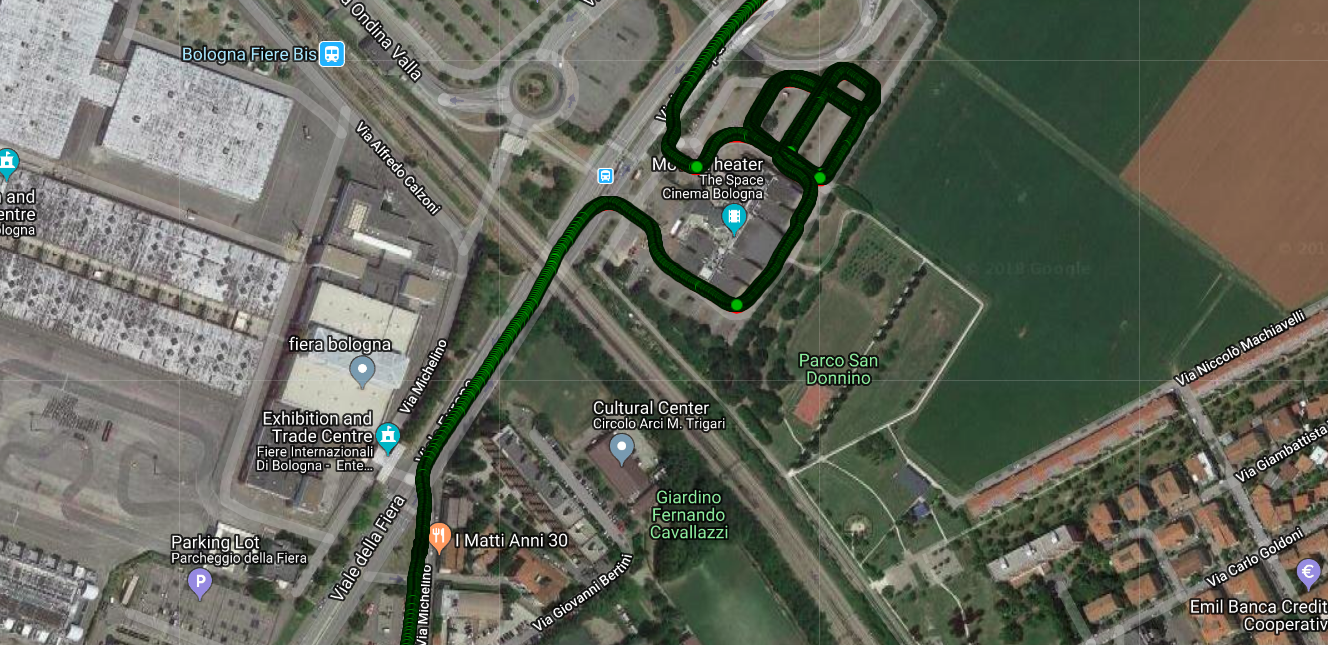
\includegraphics[width=\textwidth]{parking_map.png}
\caption{Path traveled by a car with a box installed, in a Bologna parking}
\end{figure}
\begin{figure}[H]
\centering
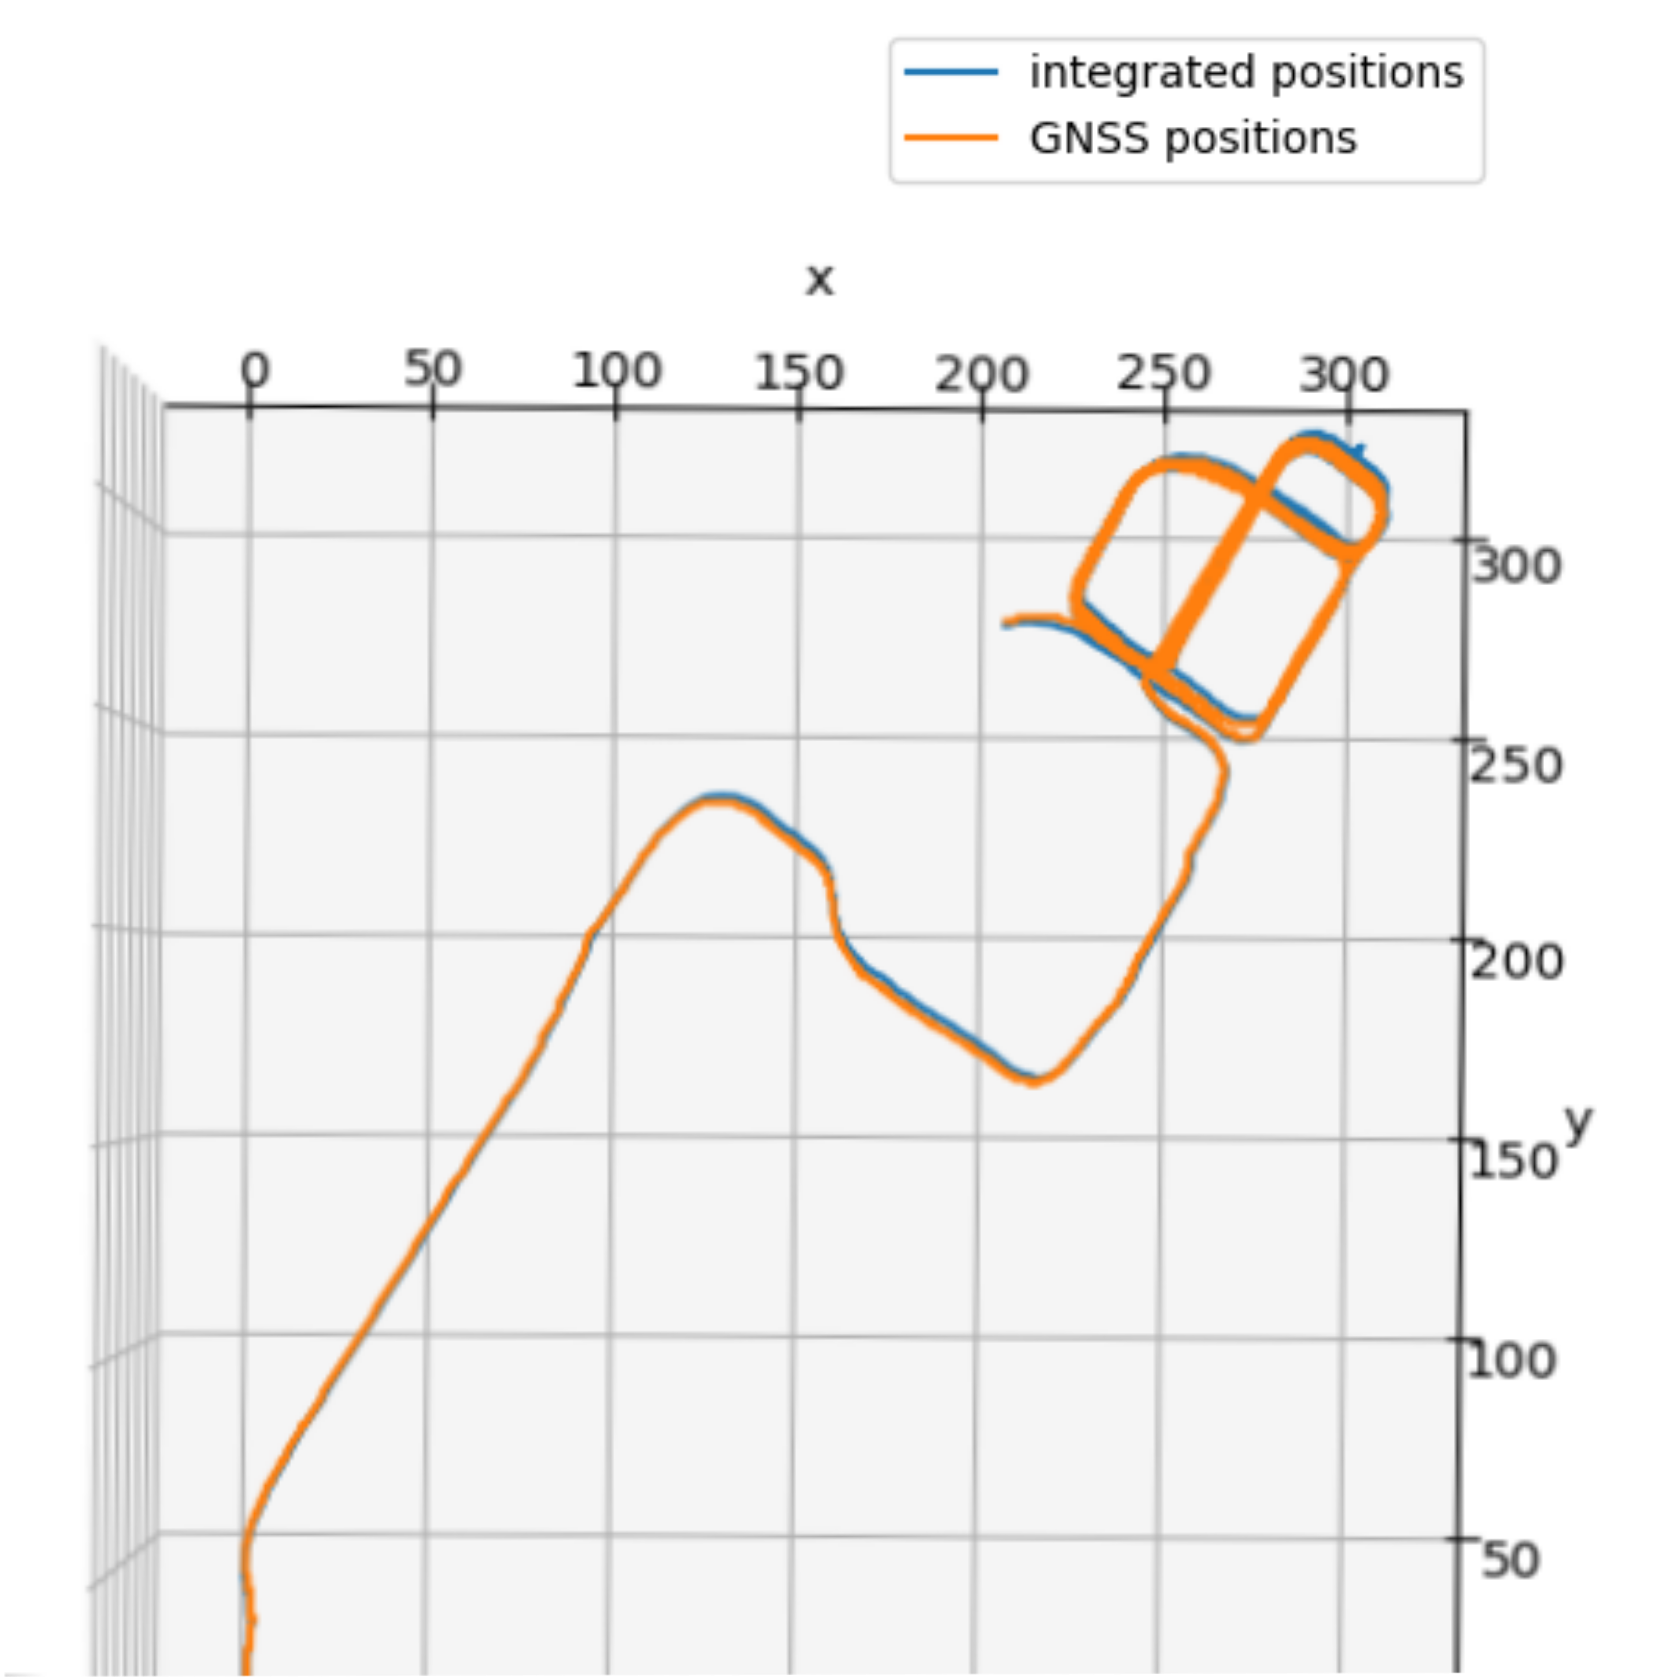
\includegraphics[scale=0.6]{parking_3d.png}
\caption{The same path from data registered by sensors and elaborated by the program}
\end{figure}
\begin{figure}[H]
\centering
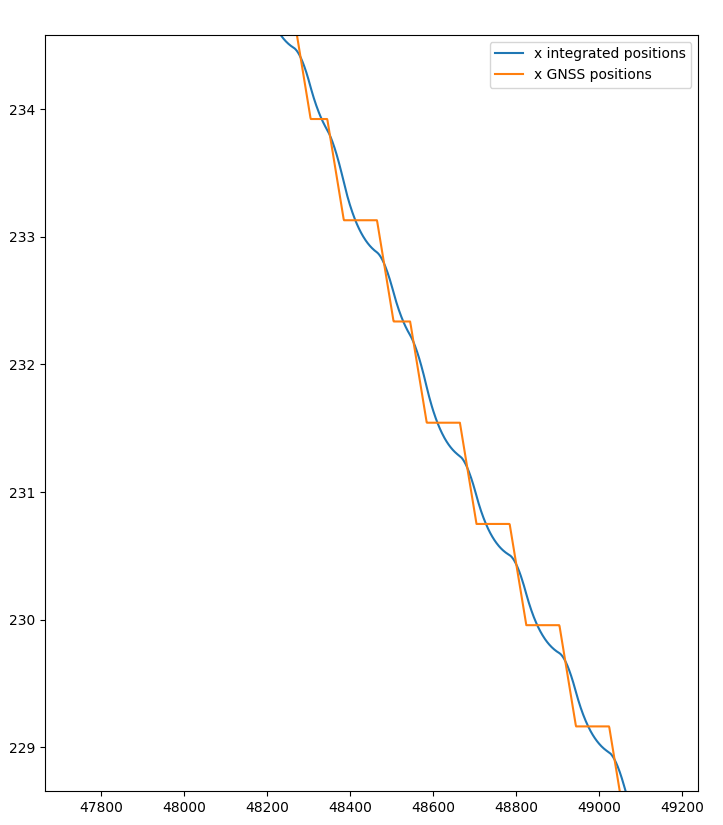
\includegraphics[width=\textwidth/2]{smooth.png}
\caption{Particular showing smoothness of integrated trajectory in respect of GNSS one}
\end{figure}

\begin{figure}[H]
\centering
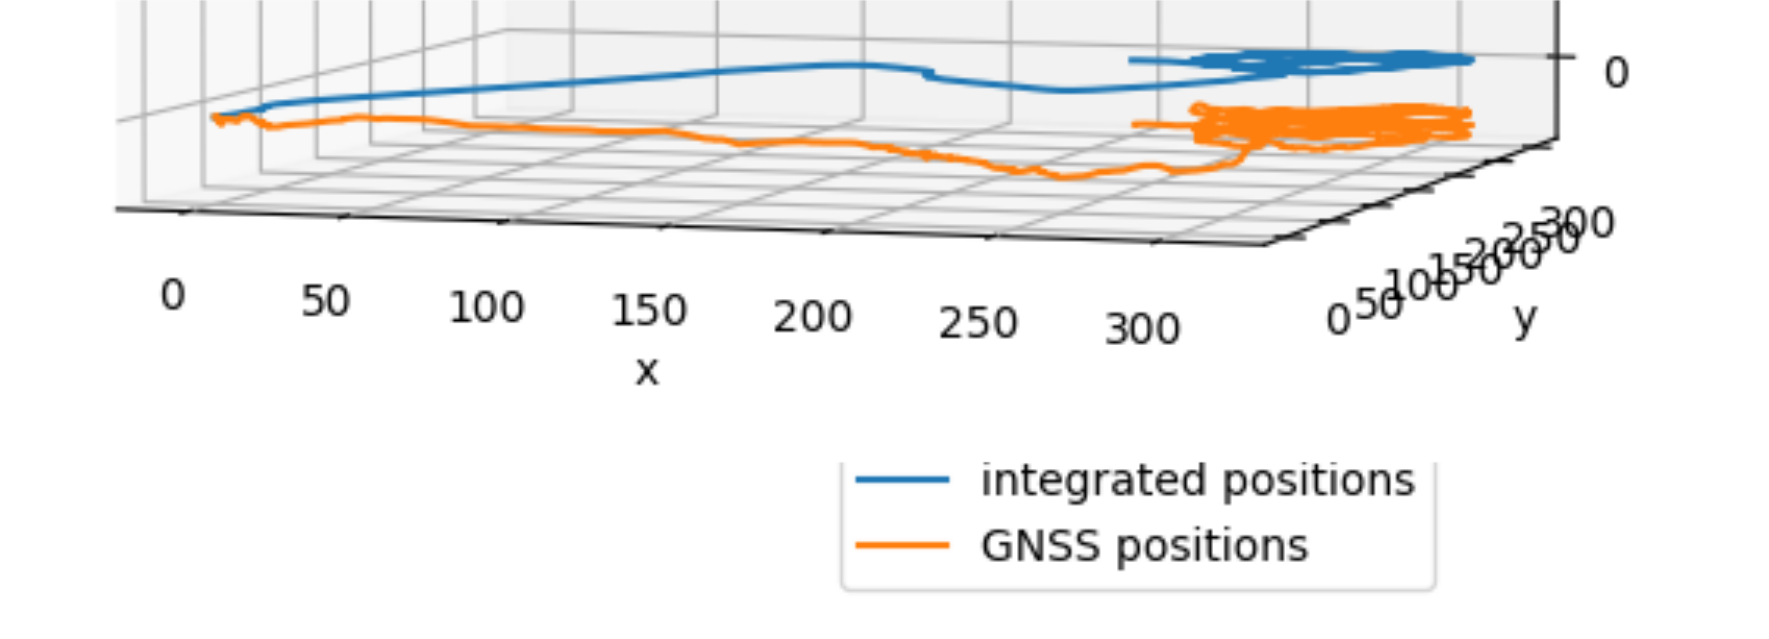
\includegraphics[width=0.8\textwidth]{parking_3d_z_different.png}
\caption{Note that GNSS and integrated path are not distant on vertical axis, this is because GNSS use altitude that is very unreadable to determine vertical position respect to accelerometer used in integrated trajectory.}
\end{figure}


